\section{Key Data Structures}

\subsection{Data Types}
\begin{frame}[fragile]
  \begin{block}{Data Types}
    \begin{center}
      \scriptsize
      \begin{tabular}{|l|l|} \hline
        \texttt{Real} & generally, a \texttt{double}, depending on \texttt{./configure} \\
                      & \\
        \texttt{Number} & a \texttt{Real} or \texttt{std::complex<Real>}, depending on \texttt{./configure} \\ 
                      & \\
        \texttt{Gradient} & a tuple of type \texttt{Number}, whose size is the spatial dimension \\ \hline
      \end{tabular}
    \end{center}
  \end{block}
  \begin{itemize}
  \item \libMesh{} can be compiled to support either real or complex-valued systems.
    \begin{lstlisting}[language=bash]
  $ ./configure --enable-complex # turns on complex number support
    \end{lstlisting}
  \item The underlying linear algebra libraries must support the requested type.
  \end{itemize}
\end{frame}

%%%%%%%%%%%%%%%%%%%%%%%%%%%%%%%%%%%%%
\subsection{The Mesh Class}
\begin{frame}[shrink]
  \frametitle{The Mesh}
  \lstinputlisting{snippets/mesh.cxx}
\end{frame}

\begin{frame}[shrink]
  \frametitle{The Mesh}
  \lstinputlisting[language=bash]{snippets/mesh.cxx.out}
\end{frame}

\begin{frame}
  \frametitle{Operations on Objects in the \texttt{Mesh}}
  \begin{block}{}
    \begin{itemize}
    \item From a \texttt{Mesh} it is trivial to access ranges of objects of interest through \emph{iterators}.
    \item Iterators are simply a mechanism for accessing a range of objects.
    \item \libMesh{} makes extensive use of \emph{predictated iterators} to access, for example,
      \begin{itemize}
        \item All elements in the mesh.
        \item The ``active'' elements in the mesh assigned to the local processor in a parallel simulation.
        \item The nodes in the mesh.
      \end{itemize}
  \end{itemize}
  \end{block}
\end{frame}

\begin{frame}[shrink]
  \frametitle{Mesh Iterators}
  \lstinputlisting{snippets/active_elem_iterators.cxx}
\end{frame}

\begin{frame}[shrink]
  \frametitle{Mesh Iterators}
  \lstinputlisting{snippets/node_iterators.cxx}
\end{frame}



%%%%%%%%%%%%%%%%%%%%%%%%%%%%%%%%%%%%%
\subsection{The EquationSystems Class}
\begin{frame}
  \frametitle{EquationSystems}
  \begin{block}{}
    \begin{itemize}
      \item The \texttt{Mesh} is a discrete representation of the geometry for a problem.
      \item For a given \texttt{Mesh}, there can be an \texttt{EquationSystems} object, which represents one or more coupled system of equations posed on the \texttt{Mesh}.
        \begin{itemize}
          \item There is only one \texttt{EquationSystems} object per \texttt{Mesh} object.
          \item The \texttt{EquationSystems} object can hold many \texttt{System} objects, each representing a logical system of equations.
        \end{itemize}
      \item High-level operations such as solution input/output is usually handled at the \texttt{EquationSystems} level.
    \end{itemize}
  \end{block}
\end{frame}

\begin{frame}[shrink]
  \frametitle{EquationSystems}
  \lstinputlisting{snippets/es.cxx}
\end{frame}

\begin{frame}[shrink]
  \frametitle{EquationSystems}
  \lstinputlisting[language=bash]{snippets/es.cxx.out}
\end{frame}
 



%%%%%%%%%%%%%%%%%%%%%%%%%%%%%%%%%%%%%
\subsection{The Elem Class}
\begin{frame}
  \frametitle{Elements}
  \begin{block}{}
    \begin{itemize}
      \item The \texttt{Elem} base class defines a geometric element in \libMesh{}.
      \item An \texttt{Elem} is defined by \texttt{Node}s, Edges (2D,3D) and Faces (3D).
      \item An \texttt{Elem} is sufficiently rich that in many cases it is the only argument required to provide to a function.
    \end{itemize}
  \end{block}
\end{frame}

\begin{frame}[shrink]
  \frametitle{Elements}
  \lstinputlisting{snippets/elem.cxx}
\end{frame}

 

%%%%%%%%%%%%%%%%%%%%%%%%%%%%%%%%%%%%%
\subsection{The \texttt{Node} Class}
\begin{frame}
  \frametitle{Nodes}
  \begin{block}{}
    \begin{itemize}
      \item \texttt{Node}s define spatial locations in arbitrary dimensions.
      \item Logically, a \texttt{Node} is a point in \emph{N}-space plus metadata:
        \begin{itemize}
          \item Global ID.
          \item Processor ownership.
          \item Degree of freedom indexing data.
        \end{itemize}
    \end{itemize}
  \end{block}
\end{frame}

\begin{frame}
  \frametitle{Nodes}
  \begin{center}
    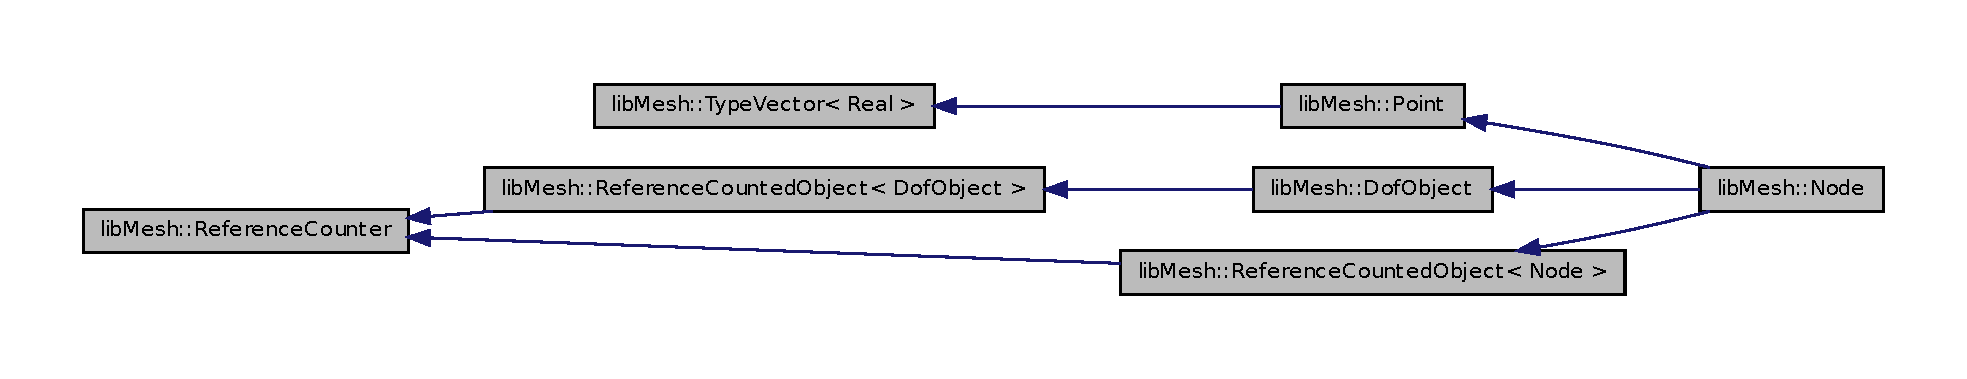
\includegraphics[width=0.95\textwidth]{libmesh_docs/classlibMesh_1_1Node__inherit__graph}
  \end{center}
\end{frame}

\begin{frame}
  \frametitle{Nodes}
  \lstinputlisting{snippets/node.cxx}
\end{frame}

